\section{Methods and System Implementation}
\subsection{Mechatronic System Architecture and Asynchronous Execution}
The experimental platform comprised an Omega.7 force-feedback master device, a seven-degree-of-freedom Franka Panda robot, a Franka Hand gripper \cite{ref26}, an Intel RealSense D435i camera, and a control computer (Fig.~\ref{fig:1}). The D435i provided 424 $\times$ 240-pixel color images at 15 fps; the depth stream was not used. The control computer ran visual detection, the nominal 200-Hz supervisory teleoperation update, parameter configuration, haptic rendering, gripper control, and data logging.

\begin{figure}[!t]
\centering
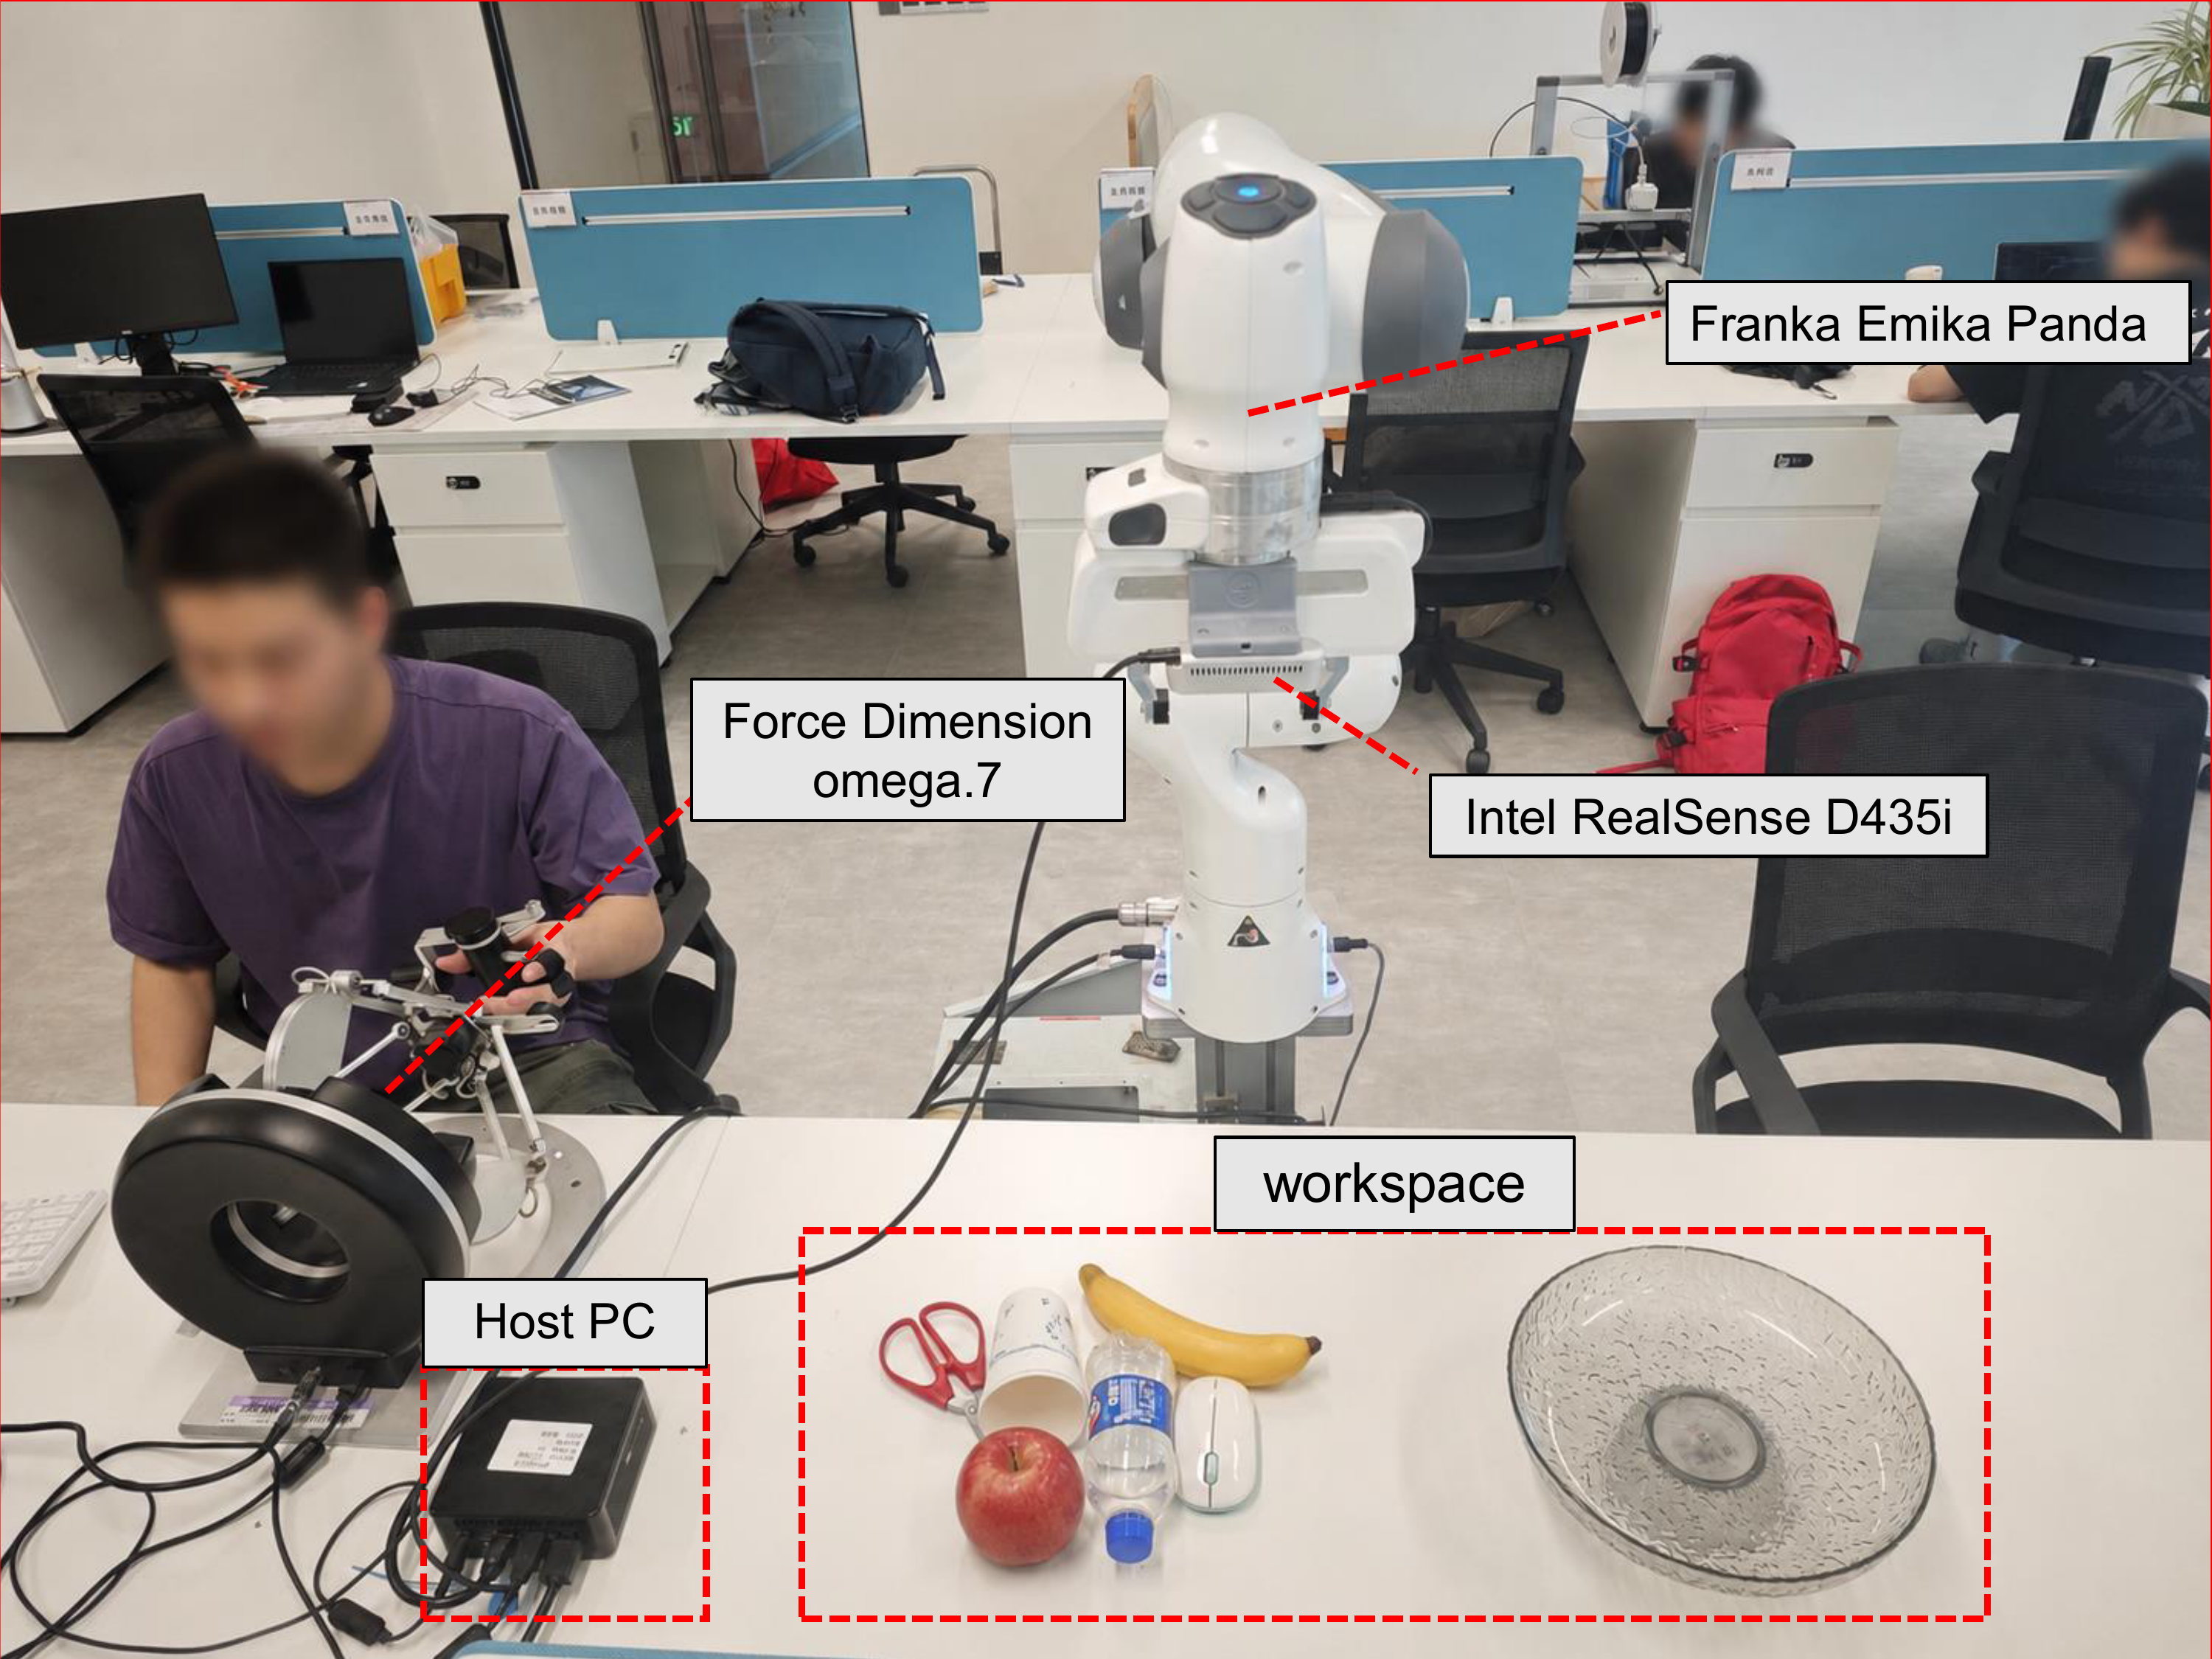
\includegraphics[width=\columnwidth]{fig1.png}
\caption{Experimental teleoperation platform showing the Omega.7 master device, Franka Panda robot, Intel RealSense D435i camera, host computer, and object workspace. The Franka Hand gripper is mounted at the Panda end effector.}
\label{fig:1}
\end{figure}

Figure~\ref{fig:2} illustrates the timing relationships within this multi-rate asynchronous software architecture.

\begin{figure*}[!t]
\centering
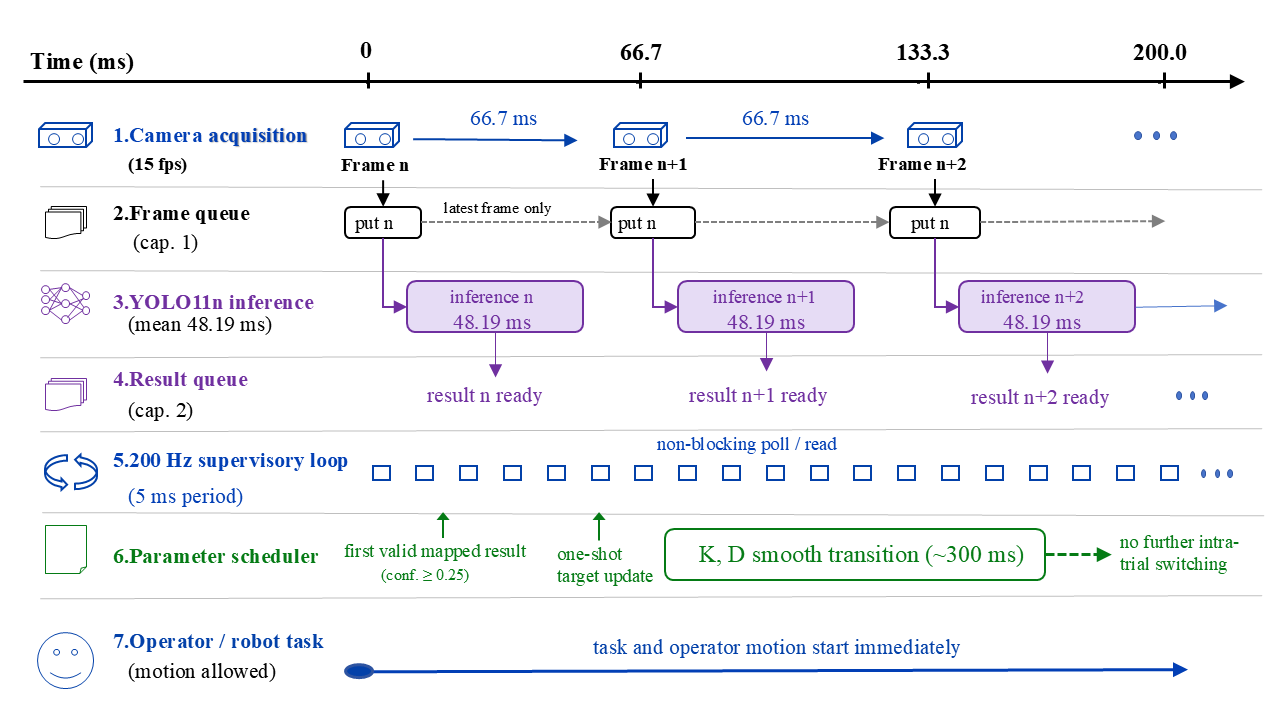
\includegraphics[width=\textwidth]{fig2.png}
\caption{Schematic, not-to-scale timing of the asynchronous perception--control implementation. Color frames are acquired at 15 fps and passed through a single-slot frame queue to an independent YOLO11n process. Class labels and confidence scores are returned through a two-slot result queue, which is polled without blocking by the nominal 200-Hz supervisory loop. The first valid mapped result (confidence $\geq 0.25$) triggers a one-shot target update. Translational stiffness, rotational stiffness, and the controller damping-scaling parameter are commanded to follow a smooth transition with a nominal duration of approximately 300 ms. Subsequent detections do not change the target within the same trial, while task execution and operator motion begin immediately. The schematic does not measure end-to-end trigger latency or trigger-to-contact timing.}
\label{fig:2}
\end{figure*}

RGB frames were acquired every 66.7 ms and written to a single-slot queue, preventing stale images from accumulating. YOLO11n ran in an independent process and returned class labels and confidence scores through a two-slot result queue. The nominal 200-Hz supervisory loop polled this queue every 5 ms without waiting for inference, allowing camera acquisition, perception, and operator motion to proceed in parallel. Per-image processing time was evaluated separately from the 15-fps camera sampling period, as reported in Section~4.1. Table~\ref{tab:1} summarizes the update timing, triggers, and data flow of the system modules.

\begin{table*}[!t]
\centering
\caption{Runtime characteristics and data flow of the multi-rate mechatronic system.}
\label{tab:1}
\small
\setlength{\tabcolsep}{6pt}
\renewcommand{\arraystretch}{1.16}
\begin{tabularx}{\textwidth}{@{}p{0.20\textwidth}p{0.24\textwidth}Y@{}}
\toprule
Module & Timing or trigger & Data flow \\
\midrule
Master input & 200 Hz & Omega.7 translational position and buttons $\rightarrow$ master-state update. \\
Slave control & 200 Hz & Desired pose and impedance parameters $\rightarrow$ Panda command. \\
Image acquisition & 15 fps (66.7 ms/frame) & D435i color stream $\rightarrow$ $424\times240$ color image. \\
YOLO11n inference & Asynchronous; controlled-test performance reported in Section~4.1 & Latest available image $\rightarrow$ class and confidence. \\
Strategy scheduling & First threshold-qualified detection & Class and confidence $\rightarrow$ target $\Theta(c)$. \\
Haptic rendering & 200 Hz & Force-related state $\rightarrow$ Omega.7 force command. \\
Gripper command & Button event & Gripper input and command parameters $\rightarrow$ Franka Hand command. \\
\bottomrule
\end{tabularx}
\par\smallskip
\footnotesize\textit{Note:} YOLO11n inference is executed in an independent process and does not block the supervisory loop.
\end{table*}
\subsection{Master--Slave Mapping and Implementation of the Mechatronic Channels}
Only translational motion of the Omega.7 was mapped to the Panda. The master-device position increment and desired slave position were updated as

\begin{equation}
\label{eq:master-position-increment}
\Delta\mathbf{p}_m(k)=\mathbf{p}_m(k)-\mathbf{p}_m(k-1),
\end{equation}

\begin{equation}
\label{eq:desired-slave-position}
\mathbf{p}_d(k)=\mathbf{p}_d(k-1)+S\mathbf{C}\Delta\mathbf{p}_m(k),
\end{equation}

where the position-scaling factor was $S=3.0$ and $\mathbf{C}=\mathrm{diag}(-1,-1,1)$. The desired end-effector orientation $\mathbf{R}_d$ was fixed at its prescribed value throughout each trial; active rotational input from the operator was not mapped. At a conceptual level, Cartesian impedance control acted on the six-dimensional pose error,

\begin{equation}
\label{eq:cartesian-impedance}
\mathbf{w}_c=\mathbf{K}(c)\mathbf{e}+\mathbf{D}(c)\dot{\mathbf{e}},
\end{equation}

\begin{equation}
\label{eq:stiffness-matrix}
\mathbf{K}(c)=\mathrm{diag}(K_t,K_t,K_t,K_r,K_r,K_r),
\end{equation}

where $\mathbf{e}$ contains translational error relative to $\mathbf{p}_d$ and rotational error relative to the fixed $\mathbf{R}_d$. Thus, $K_r$ changes resistance to rotational disturbances and the ability to hold the prescribed orientation; it does not scale operator-commanded rotation. Here $\mathbf{D}$ denotes the controller's effective damping action rather than an independently identified physical Cartesian damping matrix.

The slave-controller API internally generated its normalized damping action from the active diagonal stiffness matrix and a scalar API parameter denoted by $\zeta$. In the implementation convention,

\begin{equation}
\label{eq:damping-matrix}
\mathbf{D}_{\mathrm{API}}(c)=2\zeta(c)\sqrt{\mathbf{K}(c)},
\end{equation}

where the square root is applied elementwise to the diagonal entries. $\mathbf{D}_{\mathrm{API}}$ denotes the API's normalized internal construction and is not reported as a physical damping matrix in SI units. Accordingly, $\zeta$ is treated only as the dimensionless damping-scaling parameter exposed by the controller API and is not interpreted as a Cartesian critical-damping ratio, because no effective Cartesian mass or inertia matrix was identified.

For haptic rendering, the Franka internal state estimator provided the slave-side external-force estimate $\mathbf{F}_{\mathrm{ext}}$ in newtons. The baseline master-side force command along direction $i$ was

\begin{equation}
\label{eq:baseline-haptic-command}
u_{h,i}^{\mathrm{base}}=
\operatorname{sgn}\!\left(K_fF_{\mathrm{ext},i}\right)
\max\!\left(\left|K_fF_{\mathrm{ext},i}\right|-d,0\right),
\quad i\in\{x,y,z\},
\end{equation}

where $K_f$ is a dimensionless force-scaling factor and $d$ is a per-axis dead-zone threshold in newtons.

A separate positive-$z$ cue was generated solely from the Omega.7 gripper angle $\theta_{\Omega}$:

\begin{equation}
\label{eq:gripper-cue-activation}
\alpha_g=\operatorname{clip}\!\left(
\frac{\theta_{\max}-\theta_{\Omega}}
{\theta_{\max}-\theta_{\min}},0,1\right),
\end{equation}

\begin{equation}
\label{eq:gripper-cue-command}
u_g=\min\!\left(\alpha_gG_{\mathrm{cue}}F_{\mathrm{cue,max}},F_{\mathrm{cue,max}}\right),
\qquad
u_{h,z}=u_{h,z}^{\mathrm{base}}+u_g.
\end{equation}

With $G_{\mathrm{cue}}=0.3$ and $F_{\mathrm{cue,max}}=1.0$ N, the cue was $u_g=0.3\alpha_g$ N and therefore remained within $[0,0.3]$ N. It was updated during every nominal 200-Hz supervisory cycle, with a more open Omega.7 gripper producing a larger cue. This signal represents only the Omega.7 gripper aperture; it contains no measurement of Franka Hand aperture, master--slave aperture error, grasp force, or button state.

For gripper execution, $v_g$ was passed as the \texttt{speed} argument of the \texttt{grasp} API, whose remaining arguments were \texttt{width}, \texttt{force}, \texttt{epsilon\_inner}, and \texttt{epsilon\_outer}; it was also used by \texttt{move} during opening and non-grasp position adjustments. The strategy value $F_g$ specified the requested \texttt{force} argument of \texttt{grasp()} in newtons; it was not an independently measured fingertip force. The target grasp width was 0 m. After contact and successful entry into the \texttt{HOLDING} state, the grasp command was not repeatedly retransmitted; the gripper maintained the grasp internally until \texttt{stop()} and the subsequent release or opening command.

Together, the three parameter channels act on distinct elements of the teleoperation system. Panda impedance defines the slave-side response to pose error and disturbance, the Omega.7 settings determine how the estimated external force is rendered to the operator, and the Franka Hand settings govern grasp execution. The proposed method assigns these settings in parallel from a single operational strategy. Coordination therefore occurs at the strategy layer through a consistent parameter bundle; no dynamic coupling constraint or master--slave impedance-matching law is derived between channels. Haptic transparency and closed-loop fingertip-force accuracy were not evaluated.

\subsection{Object-Conditioned Strategy-Level Multi-Subsystem Parameter Configuration}
The framework uses a three-level mapping from detected object class to an operational strategy and then to a joint parameter vector,

\begin{equation}
\label{eq:strategy-vector}
\Theta(c)=\{K_t,K_r,\zeta,K_f,d,v_g,F_g\}.
\end{equation}

The strategy classes represent combined grasping risks rather than material softness alone. The apple and banana were assigned to the fragility-priority strategy because lower contact impact, closing speed, and requested grasp force were preferred to limit squeezing and deformation, while their smooth surfaces still posed a risk of slip. The paper cup and bottle were assigned to the balanced strategy. Excessive force can deform a paper cup, whereas overly low settings may produce an insecure grasp; the bottle similarly requires a compromise between gentle handling and slip resistance. The mouse and scissors were assigned to the stability-priority strategy because their smooth or irregular surfaces and transfer demands---and, for the scissors, elongated geometry---placed greater emphasis on pose retention and grasp stability. These assignments were specific to the present objects, platform, and task; the associated parameter settings are listed in Table~\ref{tab:2}.

\begin{table*}[!t]
\centering
\caption{Parameter settings for the three operational strategies. $K_t$ is in N/m, $K_r$ in N\,m/rad, $d$ in N, $v_g$ in m/s, and $F_g$ is the requested \texttt{grasp()} force in N. $\zeta$ and $K_f$ are dimensionless controller/API scaling parameters.}
\label{tab:2}
\small
\setlength{\tabcolsep}{6pt}
\renewcommand{\arraystretch}{1.16}
\begin{tabularx}{\textwidth}{@{}p{0.18\textwidth}p{0.20\textwidth}YYY@{}}
\toprule
Strategy & Assigned objects & Slave impedance & Haptic interface & Gripper \\
\midrule
Fragility-priority & Apple, banana & $K_t=50$ N/m; $K_r=5$ N\,m/rad; $\zeta=0.8$ & $K_f=0.2$; $d=0.3$ N & $v_g=0.02$ m/s; $F_g=8$ N \\
Balanced & Paper cup, bottle & $K_t=150$ N/m; $K_r=10$ N\,m/rad; $\zeta=1.0$ & $K_f=0.5$; $d=0.4$ N & $v_g=0.05$ m/s; $F_g=15$ N \\
Stability-priority & Mouse, scissors & $K_t=200$ N/m; $K_r=13$ N\,m/rad; $\zeta=1.2$ & $K_f=0.7$; $d=0.5$ N & $v_g=0.10$ m/s; $F_g=20$ N \\
\bottomrule
\end{tabularx}
\end{table*}
At run time, the first threshold-qualified result read by the supervisory loop triggered a one-time update of the parameters enabled in the active mode, after which the strategy remained locked for the rest of the trial. Translational stiffness, rotational stiffness, and the damping-scaling parameter followed a smoothstep interpolation over approximately $T_s=0.30$ s. With $\tau=\operatorname{clip}((t-t_0)/T_s,0,1)$ and $s(\tau)=3\tau^2-2\tau^3$, each interpolated quantity $q\in\{K_t,K_r,\zeta\}$ was updated as

\begin{equation}
\label{eq:smoothstep-update}
q(t)=q_0+s(\tau)(q_\mathrm{target}-q_0).
\end{equation}

The smoothstep interpolation yields continuous trajectories for $K_t$, $K_r$, and $\zeta$, with zero update rate at the start and end of the transition. It was introduced to reduce discontinuities in the commanded impedance parameters and is not interpreted as a formal transient-stability guarantee for the complete teleoperation system.

The controller recomputed $\mathbf{D}_{\mathrm{API}}$ from the current $\mathbf{K}$ and $\zeta$ during this transition. Enabled values of $K_f$, $d$, $v_g$, and $F_g$ changed immediately at the strategy event. The update was intended to occur before first contact; however, because operator motion was not gated by perception and trigger--contact timestamps were not recorded, trial-level contact-preparatory timing could not be verified.

The class-to-strategy mapping is manually engineered. Its role is not to infer physical properties directly, but to convert a recognized object condition into a constrained, repeatable operating strategy spanning three subsystems. If an existing detector already provides a stable label for a new object, that label can be added to the mapping without retraining the controller. If the detector cannot identify or distinguish the object reliably, it must be retrained or replaced before a strategy can be assigned. The present system does not automatically infer fragility, friction, or other physical attributes for an unseen class.

\begin{figure*}[!t]
\centering
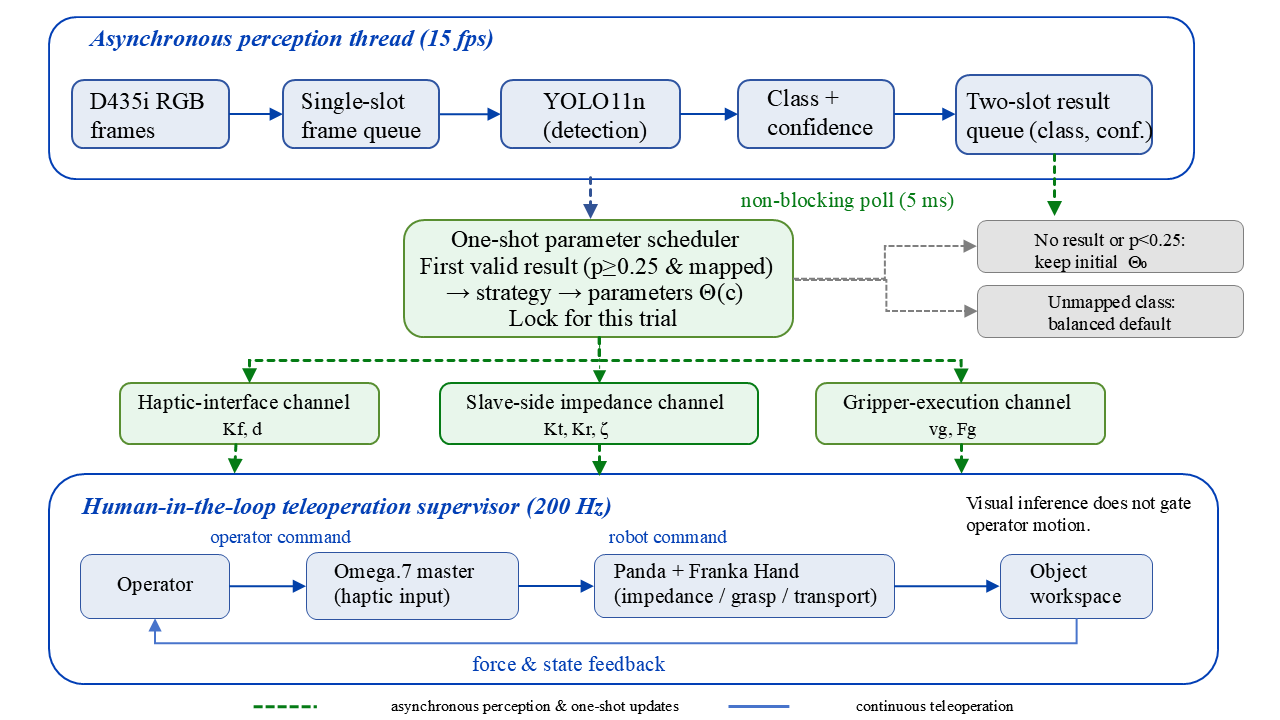
\includegraphics[width=\textwidth]{fig3.png}
\caption{Object-conditioned strategy-level parameter-bundle architecture. D435i RGB frames are processed asynchronously by YOLO11n and returned as class--confidence results through bounded queues. The 200-Hz teleoperation supervisor polls the result queue without blocking. The first mapped result with confidence $\geq 0.25$ is converted into one strategy event $\Theta(c)$, which atomically assigns the haptic-interface, slave-side impedance, and gripper-execution parameter groups and is locked for the trial. The diagram also shows the retained initial state for no or low-confidence results, the balanced default for an unmapped class, and the continuous operator--robot force/state-feedback loop. This is an implementation architecture; formal trials did not retain event-level trigger histories or synchronized trigger--contact timestamps.}
\label{fig:3}
\end{figure*}

\subsection{Experimental Modes and Parameter Rationale}
The fixed baseline vector was

\begin{equation}
\label{eq:baseline-parameter-vector}
\Theta_0=(150,\ 10,\ 1.0,\ 0.5,\ 0.3,\ 0.10,\ 20),
\end{equation}

with the same element order as $\Theta(c)$. Table 3 summarizes the five experimental conditions and the comparisons they support.

\begin{table*}[!t]
\centering
\caption{Experimental conditions, channel-update logic, and comparison roles for the five modes.}
\label{tab:3}
\scriptsize
\setlength{\tabcolsep}{4pt}
\renewcommand{\arraystretch}{1.20}
\begin{tabularx}{\textwidth}{@{}p{0.13\textwidth}p{0.23\textwidth}>{\centering\arraybackslash}p{0.105\textwidth}>{\centering\arraybackslash}p{0.105\textwidth}>{\centering\arraybackslash}p{0.105\textwidth}Y@{}}
\toprule
Mode & Visual cue / selection & Slave impedance & Haptic interface & Gripper execution & Comparison role \\
\midrule
A: Fixed-parameter baseline & None & --- & --- & --- & Fixed-parameter baseline. \\
B: Manual-selection workflow baseline & No visual cue; operator selects a complete strategy after timing starts. & Manual & Manual & Manual & Workflow baseline; timing includes manual identification and selection. \\
C: Joint parameter-bundle configuration & Class, strategy, confidence, and colored bounding box & Auto & Auto & Auto & Proposed architecture; C--D compares the full bundle with the displayed fixed-parameter condition, and C--E compares the full bundle with impedance-only reconfiguration. \\
D: Visual-semantic display with fixed parameters & Same as C & --- & --- & --- & Isolates the visual-semantic display with fixed parameters. \\
E: Impedance-only reconfiguration & Same as C & Auto & --- & --- & Isolates impedance-only reconfiguration. \\
\bottomrule
\end{tabularx}
\par\smallskip
\footnotesize\textit{Note:} Auto denotes a one-shot update after the first valid visual detection; Manual denotes manual strategy selection after timing starts; --- retains the initialized setting. In modes C--E, no detection or confidence below 0.25 retains the initialized state. A detected class without an explicit mapping invokes the balanced strategy; in mode D, the visual-semantic output is displayed while $\Theta_0$ is retained. Vision is not used in modes A and B. The C--E contrast changes the haptic-interface and gripper parameter groups together and therefore does not identify their individual effects or an interaction between them.
\end{table*}
The visual display remained active throughout all formal trials in modes C--E.

The three strategies were represented by discrete operating points. Before formal data collection, two researchers qualitatively screened candidate operating points on representative objects. Settings associated with sustained oscillation, noticeable haptic discomfort, grasp failure, or visible object damage were excluded, and the three final operating points were fixed before the 135 formal trials. The fragility-priority point used 50 N/m translational stiffness, 8 N requested grasp force, and 0.02 m/s gripper speed to reduce contact and gripper-closing severity. The balanced point used 150 N/m, 15 N, and 0.05 m/s to avoid both excessive deformation and unreliable holding. The stability-priority point used 200 N/m, 20 N, and 0.10 m/s to favor pose retention and transfer stability. Table~\ref{tab:4} summarizes the parameter effects, engineering constraints, and selected levels. These operating points were selected qualitatively for the present setup and should not be interpreted as material-specific damage limits.

\begin{table*}[!t]
\centering
\caption{Parameter design space, engineering constraints, and selected levels.}
\label{tab:4}
\small
\setlength{\tabcolsep}{5pt}
\renewcommand{\arraystretch}{1.16}
\begin{tabularx}{\textwidth}{@{}p{0.18\textwidth}Yp{0.27\textwidth}p{0.16\textwidth}@{}}
\toprule
Parameter & Low-to-high operational effect & Engineering constraint & Selected levels \\
\midrule
Slave impedance: $K_t$ & Greater translational compliance and lower impact $\rightarrow$ greater positional stability. & No sustained oscillation during qualitative screening. & 50 / 150 / 200 N/m \\
Slave impedance: $K_r$ & Greater rotational compliance about the fixed desired orientation $\rightarrow$ greater resistance to rotational disturbance. & No sustained oscillation during qualitative screening. & 5 / 10 / 13 N\,m/rad \\
Slave impedance: $\zeta$ & Lower $\rightarrow$ higher controller damping scaling. & Avoid sustained oscillation and excessive sluggishness. & 0.8 / 1.0 / 1.2 \\
Haptic interface: $K_f$ & Weaker $\rightarrow$ stronger rendered external-force cue. & Acceptable Omega.7 response. & 0.2 / 0.5 / 0.7 \\
Haptic interface: $d$ & Greater sensitivity to small forces $\rightarrow$ greater suppression of small signals. & Haptic-interface jitter and noise. & 0.3 / 0.4 / 0.5 N \\
Gripper: $v_g$ & Lower-impact motion $\rightarrow$ faster grasp establishment. & Franka Hand execution range. & 0.02 / 0.05 / 0.10 m/s \\
Gripper: $F_g$ & Lower $\rightarrow$ higher requested grasp force. & Franka Hand force setting. & 8 / 15 / 20 N \\
\bottomrule
\end{tabularx}
\end{table*}
\subsection{Execution Procedure}
\textbf{Algorithm 1: Object-conditioned strategy-level parameter scheduling}

\begin{enumerate}
\item Load the mode-specific initialization in Table 3 and start the nominal 200-Hz supervisory update; launch the visual process only in modes C--E.
\item Run object detection asynchronously. The supervisory thread polls the results without blocking and checks the confidence threshold.
\item If no detection meets the threshold, retain the initialized state. If the detected label has no explicit class-to-strategy entry, assign the balanced default strategy.
\item Use the first threshold-qualified strategy to update the parameter channels enabled by the current mode. Interpolate $K_t$, $K_r$, and the controller parameter $\zeta$ over approximately 300 ms and update the enabled haptic-interface and gripper settings immediately.
\item Lock the selected strategy for the remainder of the trial and continue teleoperation, haptic rendering, and gripper execution without further visual switching.
\item Record the active parameter state, task trajectory, duration, and outcome, and reset the system after the prescribed terminal procedure.
\end{enumerate}
\subsection{Bounded Fallback and Safety Measures}
A misclassification as another known class invoked the strategy assigned to that class. A detected label without an explicit mapping invoked the balanced default strategy, whereas a missing or low-confidence detection caused no update. Every fallback outcome was confined to one of the three predefined parameter sets, although a bounded parameter set may still be inappropriate for a misclassified object. Per-trial visual events were outside the formal logging scope, so misclassifications and default-branch activations were not individually recorded.

In addition to these software fallbacks, robot collision detection, Franka Hand force settings, zero-force commands on exit, a standardized initial pose, and a manual emergency stop provided operational safeguards. The Omega.7 was operated using its standard driver and hardware configuration. The implemented mapping limited the additional master-gripper-aperture cue to 0.3 N. The baseline force-feedback command was transmitted without an additional software saturation layer, and saturation status was not logged.
